\documentclass[10pt,conference,letterpaper]{article}
\usepackage{times,amsmath,amsfonts,epsfig}
\usepackage{graphicx}
\usepackage{algorithm,algorithmicx,algpseudocode}
\renewcommand{\algorithmicrequire}{\textbf{Input:}}
\renewcommand{\algorithmicensure}{\textbf{Output:}}
\usepackage{color}
\usepackage{flushend}
\usepackage{multirow}
\usepackage{multicol}
\usepackage{cuted}
\usepackage{rotating}
\usepackage{caption}
\usepackage{ulem}
\usepackage[left=2.00cm, right=2.00cm, top=2.00cm, bottom=2.00cm]{geometry}

\title{Appendices}
\date{}

\begin{document}
	\maketitle
	
	\section{Preliminaries}\label{sec:preliminaries}
		Statistical divergence, also called statistical distance, measures the similarity between two or more distributions.
		Mathematically, statistical divergence is a function which describes the ``distance'' of one probability distribution to the other on a statistical manifold. Let $\mathbb{S}$ be a space of probability distributions, then a divergence is a function from $\mathbb{S}$ to non-negative real numbers: 
		\begin{equation}
		D(\cdot || \cdot): \mathbb{S} \times \mathbb{S} \rightarrow \mathbb{R^+} \cup \{0\}
		\end{equation}
		
		Divergence between two distributions $P$ and $Q$, written as $D(P||Q)$, satisfies:
	
		\begin{enumerate}
			\item $D(P||Q) \ge 0, \forall P, Q \in \mathbb{S}$
			\item $D(P||Q) = 0$, if and only if $P=Q$
		\end{enumerate}
		
		For our purposes, we do not require the function $D$ to have the property: $D(P||Q) = D(Q||P)$. But we do need it to be true that if $Q$ is more similar with $P$ than $U$, then $D(Q||P) < D(U||P)$. There are ways to calculate divergence,	several frequently used divergence metrics are as follows:
	
		\subsection{Kullback-Leibler Divergence}
			Let $P,Q$ be discrete probability distributions, $Q(x)=0$ implies $P(x)=0$ for $\forall x$, the \textit{Kullback-Leibler Divergence} from $Q$ to $P$ is defined to be:
			
			\begin{equation}
				KLD(P||Q) = \sum_{Q(x)\ne 0} P(x)log\Big(\frac{P(x)}{Q(x)}\Big)
			\end{equation}
			
			For $P,Q$ being continuous distributions:
			
			\begin{equation}
				KLD(P||Q) = \int_{q(x) \ne 0} p(x)log\frac{p(x)}{q(x)}dx
			\end{equation}
	
		\subsection{Jensen-Shannon Divergence}
			Let $P,Q$ be discrete probability distributions, \textit{Jensen-Shannon Divergence} between $P$ and $Q$ is defined to be:
			\begin{equation}
				JSD(P||Q) = \frac{1}{2}KLD(P||M) + \frac{1}{2}KLD(Q||M)
			\end{equation}
			where $\displaystyle M = \frac{1}{2}(P+Q)$.
			
			A more generalized form is defined to be:
			\begin{equation}
				JSD(P_1, \dots, P_n) = H\Big(\sum_{i=1}^n\pi_i P_i\Big) - \sum_{i=1}^n\pi_iH(P_i)
			\end{equation}
			where $H$ is Shannon Entropy, $\displaystyle M = \sum_{i=1}^{n}\pi_iP_i$ and $\displaystyle \sum_{i=1}^{n}\pi_i = 1$.
			
			Especially, if $\displaystyle \pi_i = \frac{1}{n}$, then:
			\begin{equation}
				JSD(P_1, \dots, P_n) = \frac{1}{n}\sum_{i=1}^{n}KLD(P_i||M)
			\end{equation}
			Jensen-Shannon divergence has some fine properties:
			\begin{enumerate}
				\item $JSD(P||Q) = JSD(Q||P), \forall P, Q\in \mathbb{S}$.
				\item $0 \le JSD(P_1, \dots, P_n) \le log_k(n)$. If a $k$ based algorithm is adopted.
				\item To calculate $JSD(P||Q)$, it need not necessarily to be true that $Q(x)=0$ implies $P(x)=0$.
			\end{enumerate}
		
		\subsection{Bhattacharyya Distance}
			Let $P,Q$ be discrete probability distributions over same domain $X$, \textit{Bhattacharyya Distance} between $P$ and $Q$ is defined to be:
		
			\begin{equation}
				BD(P||Q) = -ln\Big(\sum_{x\in X}\sqrt{P(x)Q(x)}\Big)
			\end{equation}
			
		\subsection{Hellinger Distance}
			Let $P,Q$ be discrete probability distributions, \textit{Hellinger Distance} between $P$ and $Q$ is defined to be:
		
			\begin{equation}
				HD(P||Q) = \frac{1}{\sqrt{2}}\sqrt{\sum_x\bigg(\sqrt{P(x)} - \sqrt{Q(x)}\bigg)^2}
			\end{equation}
		
		\subsection{Kolmogorov-Smirnov Statistic}
			Let $P,Q$ be discrete one-dimensional probability distributions, $CDF_P$ and $CDF_Q$ are their cumulative probability functions respectively, \textit{Kolmogorov-Smirnov Statistic} between $P$ and $Q$ is defined to be:
			
			\begin{equation}
				KSS(P||Q) = \sup_x | CDF_P(x) - CDF_Q(x) |
			\end{equation}
			
	\section{Adaptive Threshold Calculation}
		Suppose:
		\begin{align}
			PDF_normal(x) &\approx \mathcal{N}(\mu_n, \sigma_n)\\
			PDF_anomalous(x) &\approx \mathcal{N}(\mu_a, \sigma_a)
		\end{align}
		
		\begin{align}\label{equ:equal-weight}
			T &= \mathop{\arg\min}_{T} \int_{0}^{T}PDF_{a}(x)dx +
			\int_{T}^{\sup(D)}PDF_{n}(x)dx \nonumber\\
			& \approx \mathop{\arg\min}_{T}
			\int_{-\infty}^{T}
			\frac{e^{-\frac{(x - \mu_a)^2}{2\sigma_a^2}}}{\sqrt{2\pi} \sigma_a}dx
			+ \int_{T}^{+\infty}
			\frac{e^{-\frac{(x - \mu_n)^2}{2\sigma_n^2}}}{\sqrt{2\pi} \sigma_n}dx \nonumber\\
			& = \begin{cases}
				\displaystyle
				\frac{1}{\sigma_a^2 - \sigma_n^2}\left[(\sigma_a^2\mu_n - \sigma_n^2\mu_a) \pm \sigma_a\sigma_n\sqrt{(\mu_a - \mu_n)^2 + 2(\sigma_a^2 - \sigma_n^2)ln\frac{\sigma_a}{\sigma_n}}\right], & \sigma_a \ne \sigma_n\\
				\displaystyle \frac{\mu_n + \mu_a}{2}, & \sigma_a = \sigma_n
			\end{cases}
		\end{align}
		
		Note: when $\sigma_a \ne \sigma_n$, keep the root s.t. $\displaystyle \frac{T - \mu_a}{\sigma_a^3}e^{-\frac{(T - \mu_a)^2}{2\sigma_a^2}} < \frac{T - \mu_n}{\sigma_n^3}e^{-\frac{(T - \mu_n)^2}{2\sigma_n^2}}$
		
		\begin{align}\label{equ:linear-weight}
			T & = \mathop{\arg\min}_{T} \alpha\int_{0}^{T}PDF_{a}(x)dx +
			(1-\alpha)\int_{T}^{\sup(D)}PDF_{n}(x)dx\nonumber\\
			& \approx \mathop{\arg\min}_{T}
			\alpha\int_{-\infty}^{T}
			\frac{e^{-\frac{(x - \mu_a)^2}{2\sigma_a^2}}}{\sqrt{2\pi} \sigma_a}dx
			+ 
			(1-\alpha)\int_{T}^{+\infty}
			\frac{e^{-\frac{(x - \mu_n)^2}{2\sigma_n^2}}}{\sqrt{2\pi} \sigma_n}dx\nonumber\\
			& = \begin{cases}
				\displaystyle
				\frac{1}{\sigma_a^2 - \sigma_n^2}\left[(\sigma_a^2\mu_n - \sigma_n^2\mu_a) \pm \sigma_a\sigma_n\sqrt{(\mu_a - \mu_n)^2 + 2(\sigma_a^2 - \sigma_n^2)ln\frac{(1 - \alpha)\sigma_a}{\alpha\sigma_n}}\right], & \sigma_a \ne \sigma_n\\
				\displaystyle
				\frac{\mu_n + \mu_a}{2} + \frac{k^2ln\frac{1 - \alpha}{\alpha}}{\mu_a - \mu_n}, & \sigma_a = \sigma_n = k
			\end{cases}
		\end{align}
		
		Note: when $\sigma_a \ne \sigma_n$, keep the root s.t. $\displaystyle \frac{\alpha (T - \mu_a)}{\sigma_a^3}e^{-\frac{(T - \mu_a)^2}{2\sigma_a^2}} < \frac{(1 - \alpha) (T - \mu_n)}{\sigma_n^3}e^{-\frac{(T - \mu_n)^2}{2\sigma_n^2}}$
		
	\section{Extra Insights on Koubei Data Set}
		\begin{figure}[!t]
			\centering
			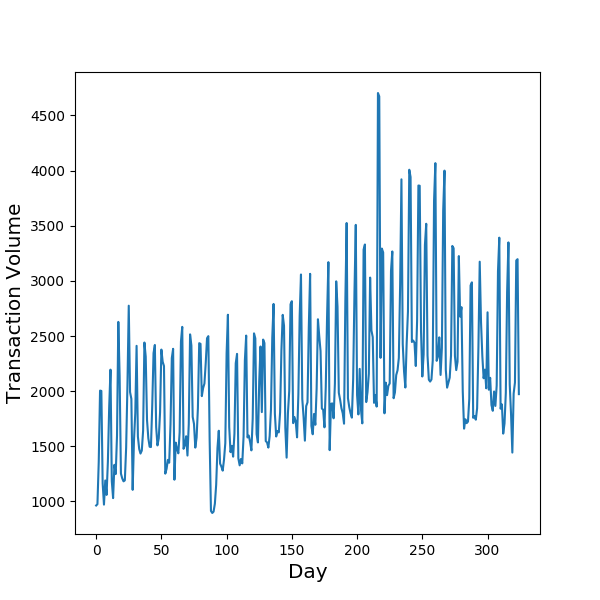
\includegraphics[width=0.5\linewidth]{fig/DailyTransactionVolume.png}
			\caption{Changing of the daily sales volume shows that environment of online sales had been changing all the time.}
			\label{fig:daily-transaction-volume}
		\end{figure}
		
		\begin{figure}[!t]
			\centering
			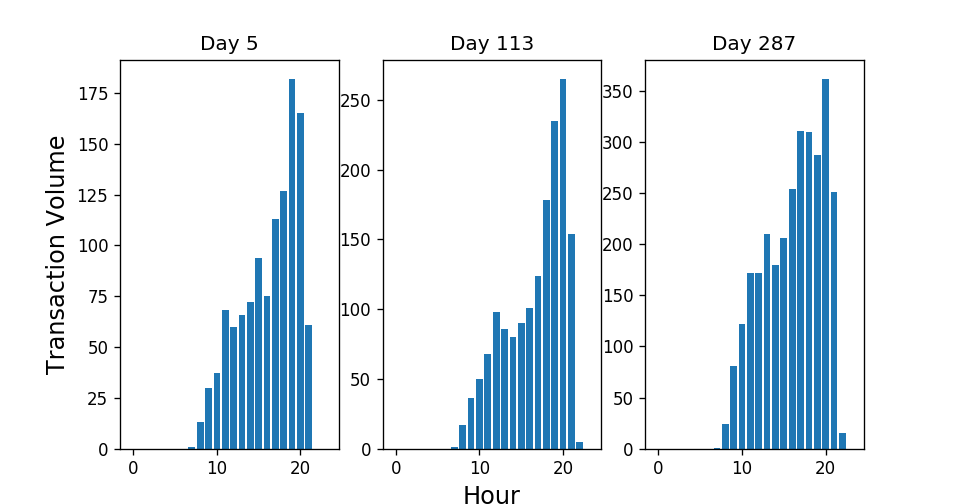
\includegraphics[width=.7\linewidth]{fig/SaleDistributions.png}
			\caption{We selected 3 days randomly and drew sales distribution by counting hourly volume. Although sales volume has changed from day to day, the shape of the distribution remain almost alike.}
			\label{fig:sale-distribution-sample}
		\end{figure}
		
		\begin{figure}[!t]
			\centering
			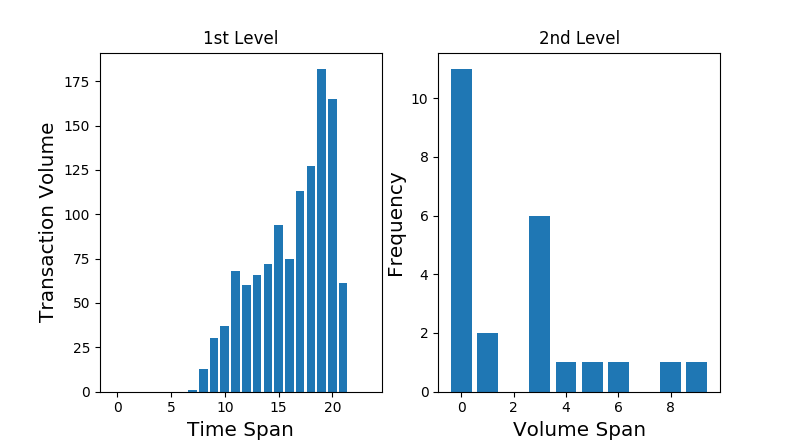
\includegraphics[width=\linewidth]{fig/HistogramExample.png}
			\caption{Examples of 1st and 2nd Level Histogram}
			\label{fig:histogram-example}
		\end{figure}
		
		\begin{figure}[!t]
			\centering
			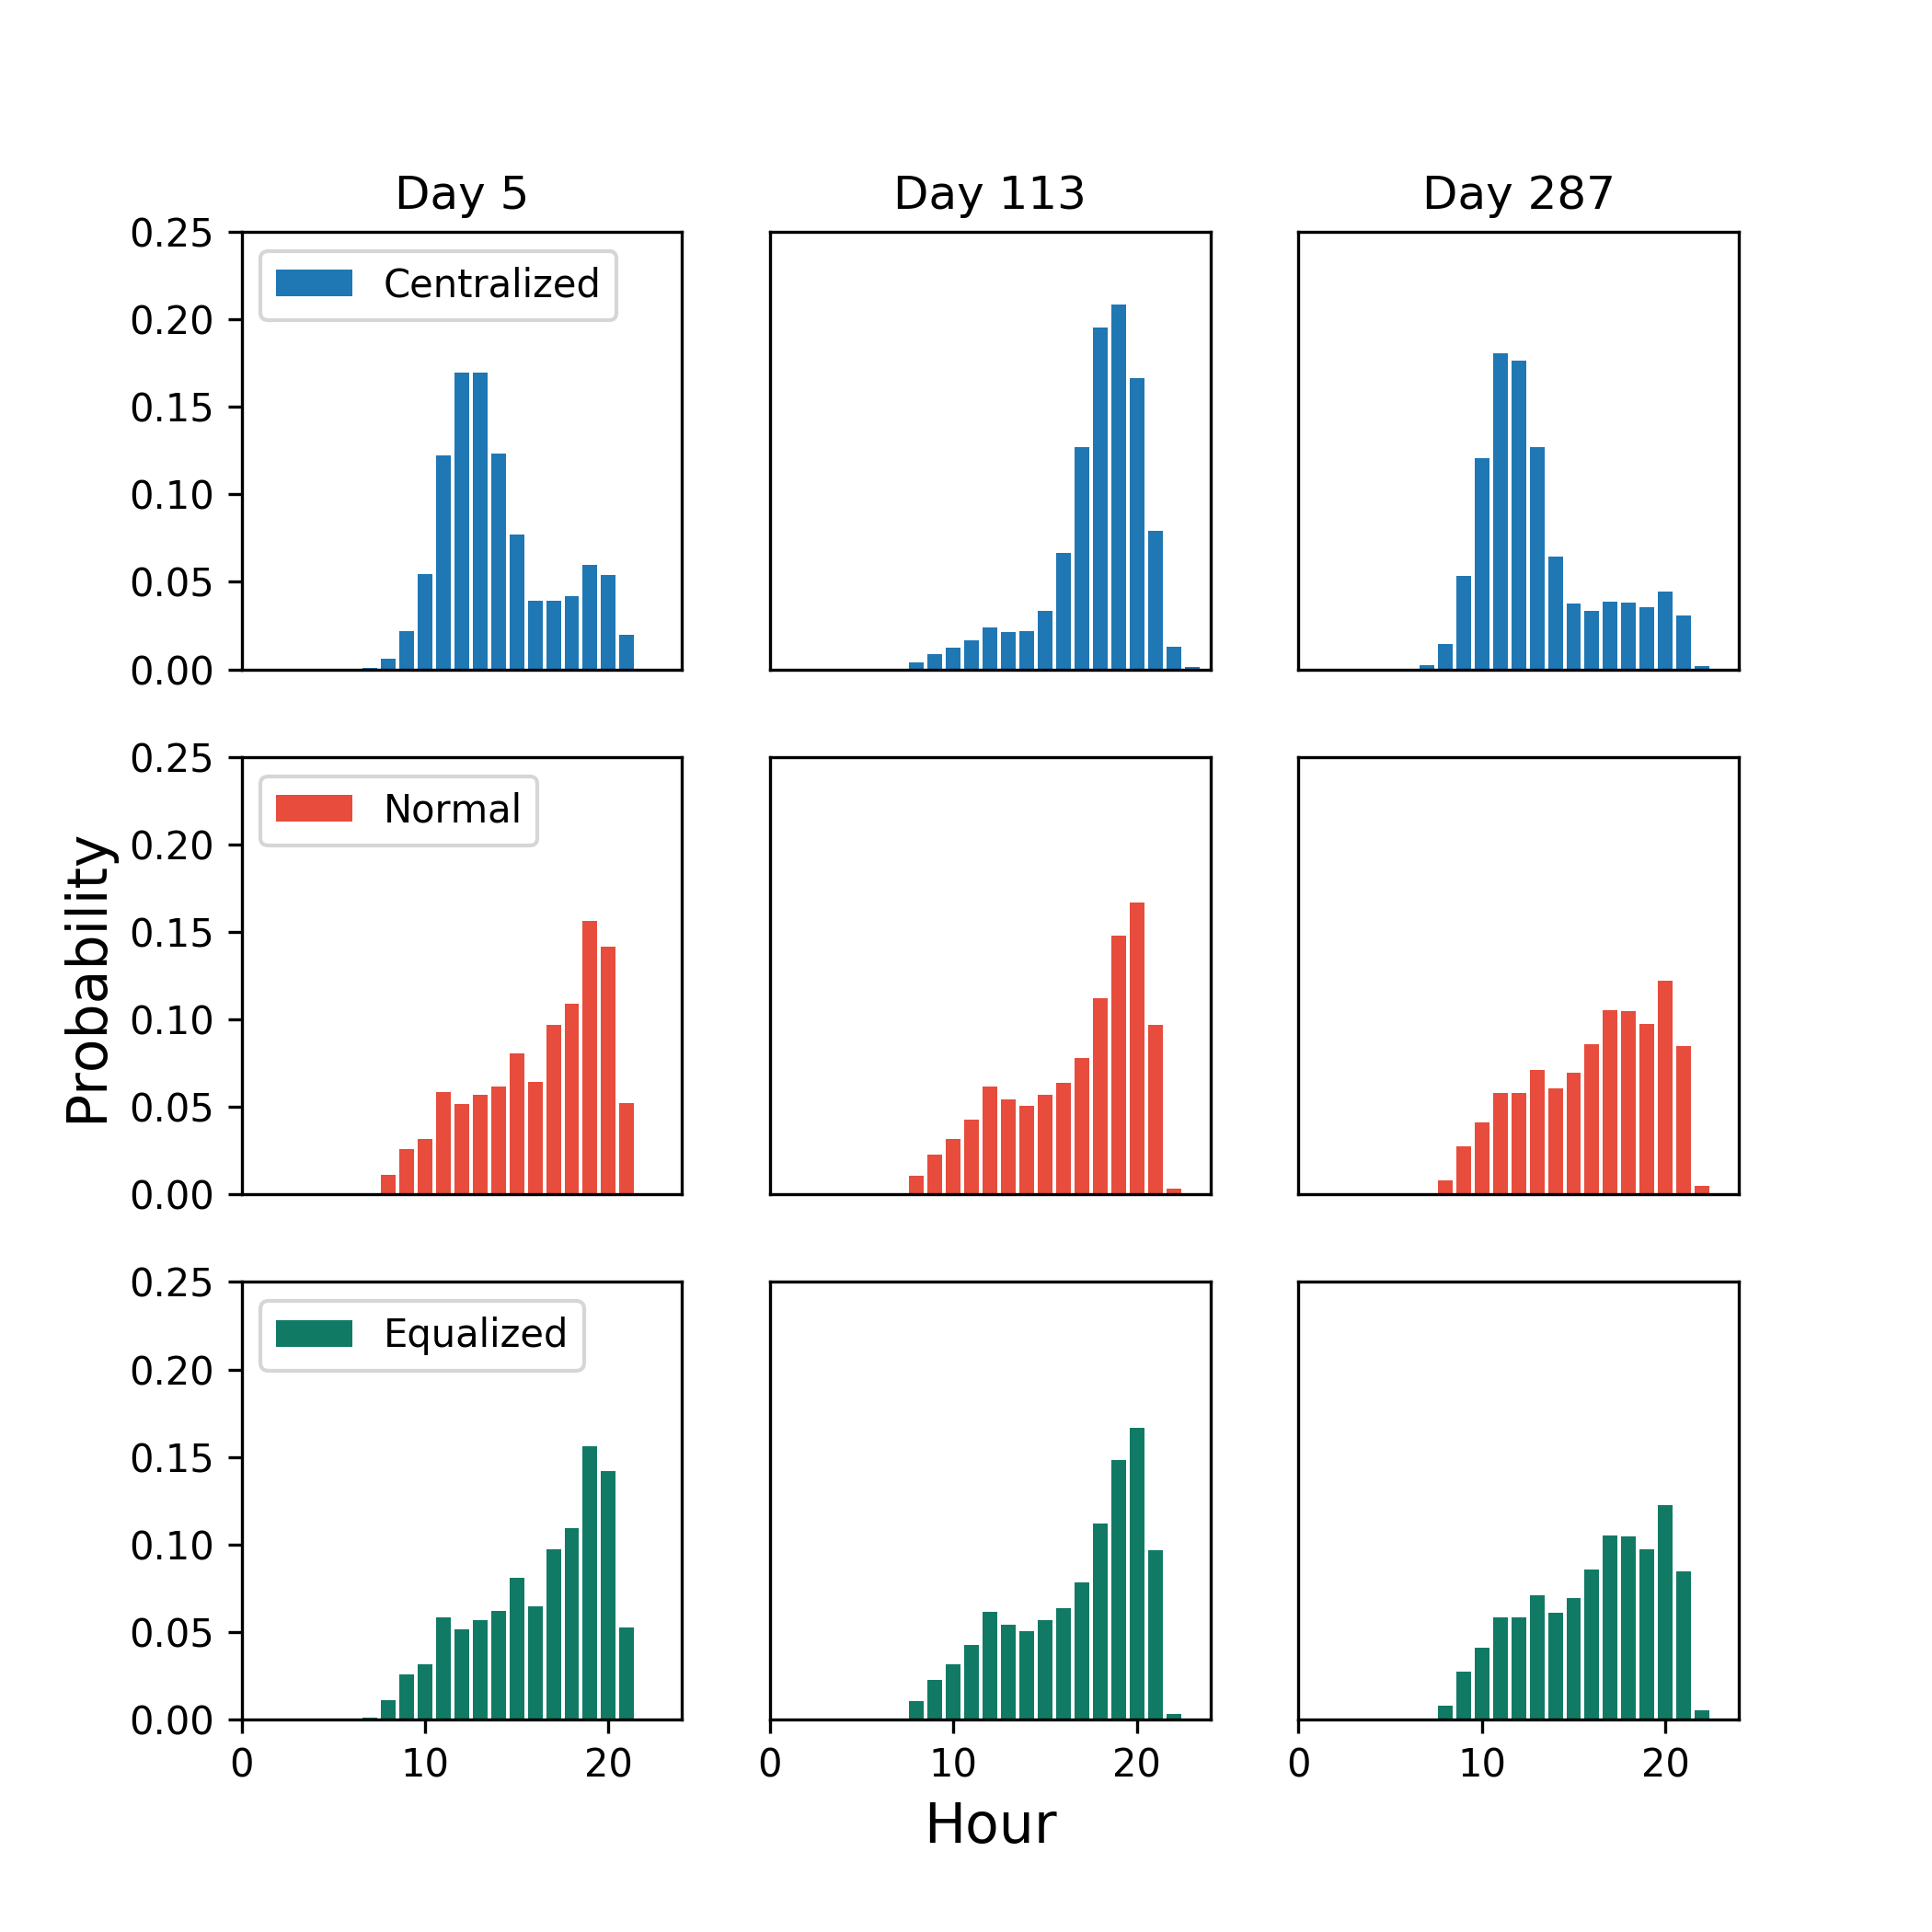
\includegraphics[width=\linewidth]{fig/Raw1stLevelHist.png}
			\caption{1st level histogram of day 5, 113 and 287, each day in a column. Distributions after centralized and equalized click farming are in 1st and 3rd rows correspondingly. And the original distributions are shown in the 2nd row.}
			\label{fig:raw-hist-1st}
		\end{figure}
		
		\begin{figure}[!t]
			\centering
			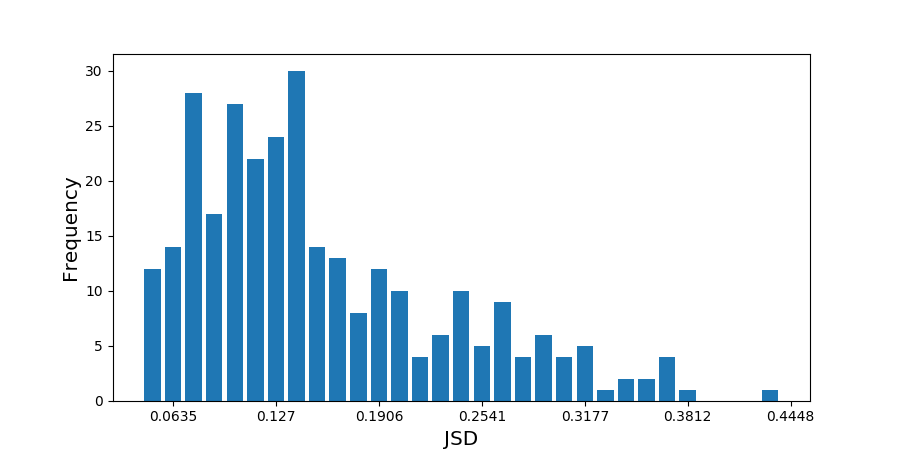
\includegraphics[width=\linewidth]{fig/JSD-Dist.png}
			\caption{Distribution of Jensen-Shannon divergence on Taobao data set(without click farming) used in the experiments.}
			\label{fig:jsd-dist}
		\end{figure}
		
	
	\section{Results on Synthetic Data Set}
		The synthetic data set was divided into four sections. First two sections contained sample sets drawn from a uniform and a Gaussian distribution respectively. The third section used a mixture of one uniform distribution and two Gaussian distributions to simulate a random-shaped distribution. Moreover, we made the random-shaped distribution drift slightly to form the last section of test data. Corresponding anomalies were drown from distributions with deviated parameters respectively.
		
		In this experiment, we tested all seven algorithms on totally synthetic data sets. Results are shown in TABLE~\ref{tab:performance-synthetic}. It shows that our technique can be applied towards any kind of distributions. And these techniques worked better under irregular distributions since difference were clearer among these. Comparison between SDD-R and static SDD-E 
		shows that adaptive thresholds provided more flexible classifiers. Results under random-shape drifting proves the efficiency of sliding windows toward drifting context.
		
		\begin{sidewaystable}
			\centering
			\caption{Performance Comparison on Synthetic Data Sets}
			\label{tab:performance-synthetic}
			\footnotesize
			\begin{tabular}{|c|c|c|c|c|c|c|c|c|c|c|c|c|c|c|c|c|}
				\hline
				\multirow{2}{*}{\textbf{}} & \multicolumn{4}{c|}{\textbf{Uniform}} & \multicolumn{4}{c|}{\textbf{Gaussian}} & \multicolumn{4}{c|}{\textbf{Random-shape}} & \multicolumn{4}{c|}{\textbf{Random-shape with Drift}} \\ \cline{2-17} 
				& \textbf{Pre(\%)} & \textbf{Rec(\%)} & \textbf{F1(\%)} & \textbf{T(ms)} & \textbf{Pre(\%)} & \textbf{Rec(\%)} & \textbf{F1(\%)} & \textbf{T(ms)} & \textbf{Pre(\%)} & \textbf{Rec(\%)} & \textbf{F1(\%)} & \textbf{T(ms)} & \textbf{Pre(\%)} & \textbf{Rec(\%)} & \textbf{F1(\%)} & \textbf{T(ms)} \\ \hline
				\textbf{SDD-R} & 10.00 & \textbf{100.00} & 18.18 & 349.42 & 24.78 & 69.20 & 36.49 & 401.82 & 10.00 & \textbf{100.00} & 18.18 & 351.65 & 9.97 & \textbf{99.00} & 18.11 & 353.65 \\ \hline
				\textbf{SDD-R+} & 22.40 & 22.40 & 22.40 & 348.49 & 34.40 & 34.40 & 34.40 & \textbf{398.02} & 58.40 & 58.40 & 58.40 & \textbf{350.87} & 1.20 & 1.20 & 1.20 & \textbf{346.67} \\ \hline
				\textbf{SDD-E Static} & 43.71 & 82.60 & 57.17 & 372.74 & 33.34 & 66.60 & 44.44 & 410.72 & 69.24 & 93.20 & 79.45 & 372.77 & 12.34 & 97.20 & 21.91 & 369.63 \\ \hline
				\textbf{SDD-E Static+} & \textbf{75.10} & 60.20 & \textbf{66.83} & 371.72 & \textbf{45.93} & 45.80 & \textbf{45.86} & 412.95 & \textbf{89.52} & 85.40 & \textbf{87.41} & 368.97 & 12.60 & 94.20 & 22.23 & 370.12 \\ \hline
				\textbf{SDD-E Dynamic} & 18.53 & 81.80 & 30.21 & 6808.58 & 20.28 & \textbf{71.40} & 31.58 & 8985.92 & 25.90 & 97.40 & 40.92 & 5881.37 & 13.44 & 97.20 & 23.61 & 5747.19 \\ \hline
				\textbf{SDD-E Dynamic+} & 27.85 & 25.60 & 26.68 & 8019.23 & 26.19 & 56.40 & 35.77 & 9197.94 & 77.60 & 79.40 & 78.49 & 6408.12 & \textbf{50.55} & 84.00 & \textbf{63.11} & 6176.57 \\ \hline
				\textbf{MGoF} & 10.94 & 4.40 & 6.28 & \textbf{347.97} & 10.08 & 51.60 & 16.87 & 571.93 & 6.40 & 13.60 & 8.70 & 440.26 & 2.75 & 11.60 & 4.45 & 509.58 \\ \hline
			\end{tabular}
			
			\begin{multicols}{2}
				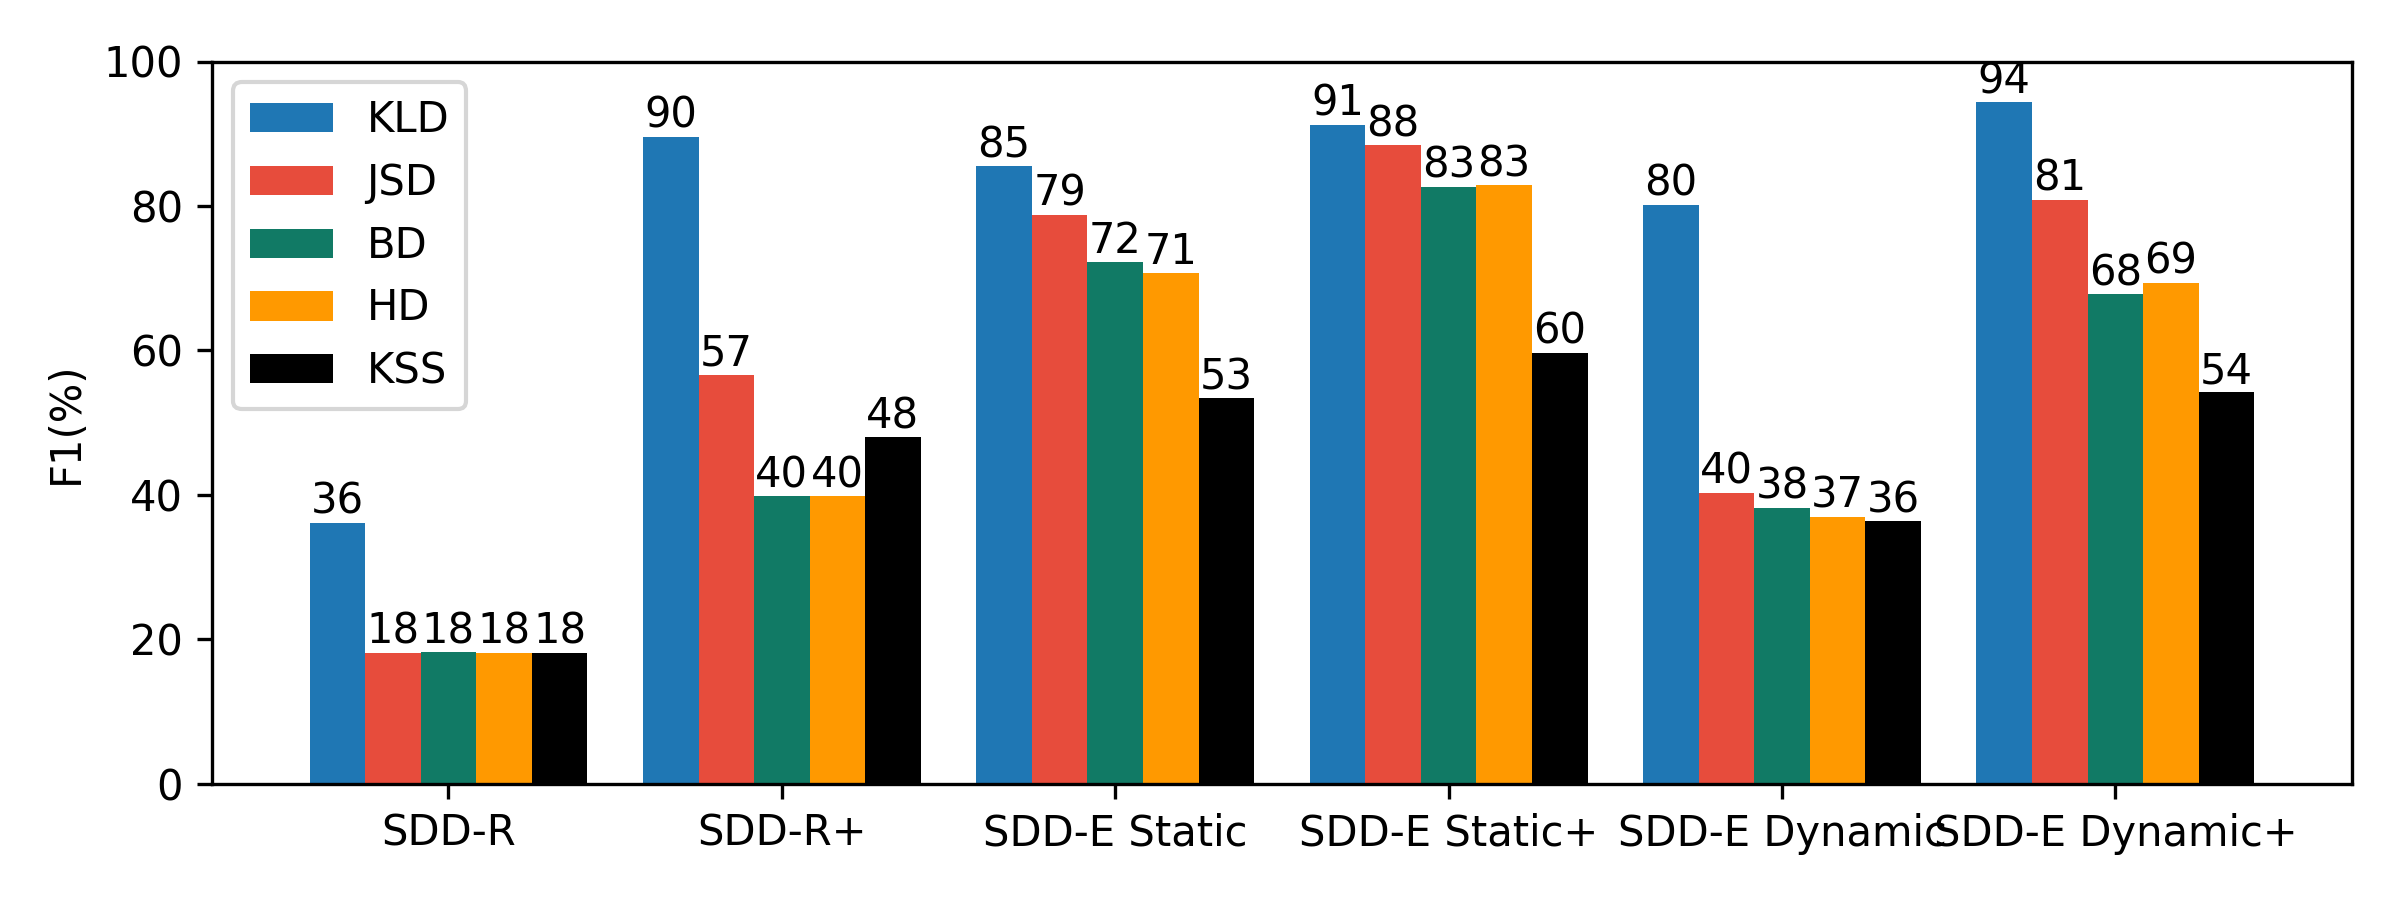
\includegraphics[width=\linewidth]{fig/F1OnDivergenceMetric.png}
				\captionof{figure}{F1 under Different Divergence Metric}
				\label{fig:divergence-metric-f1}
				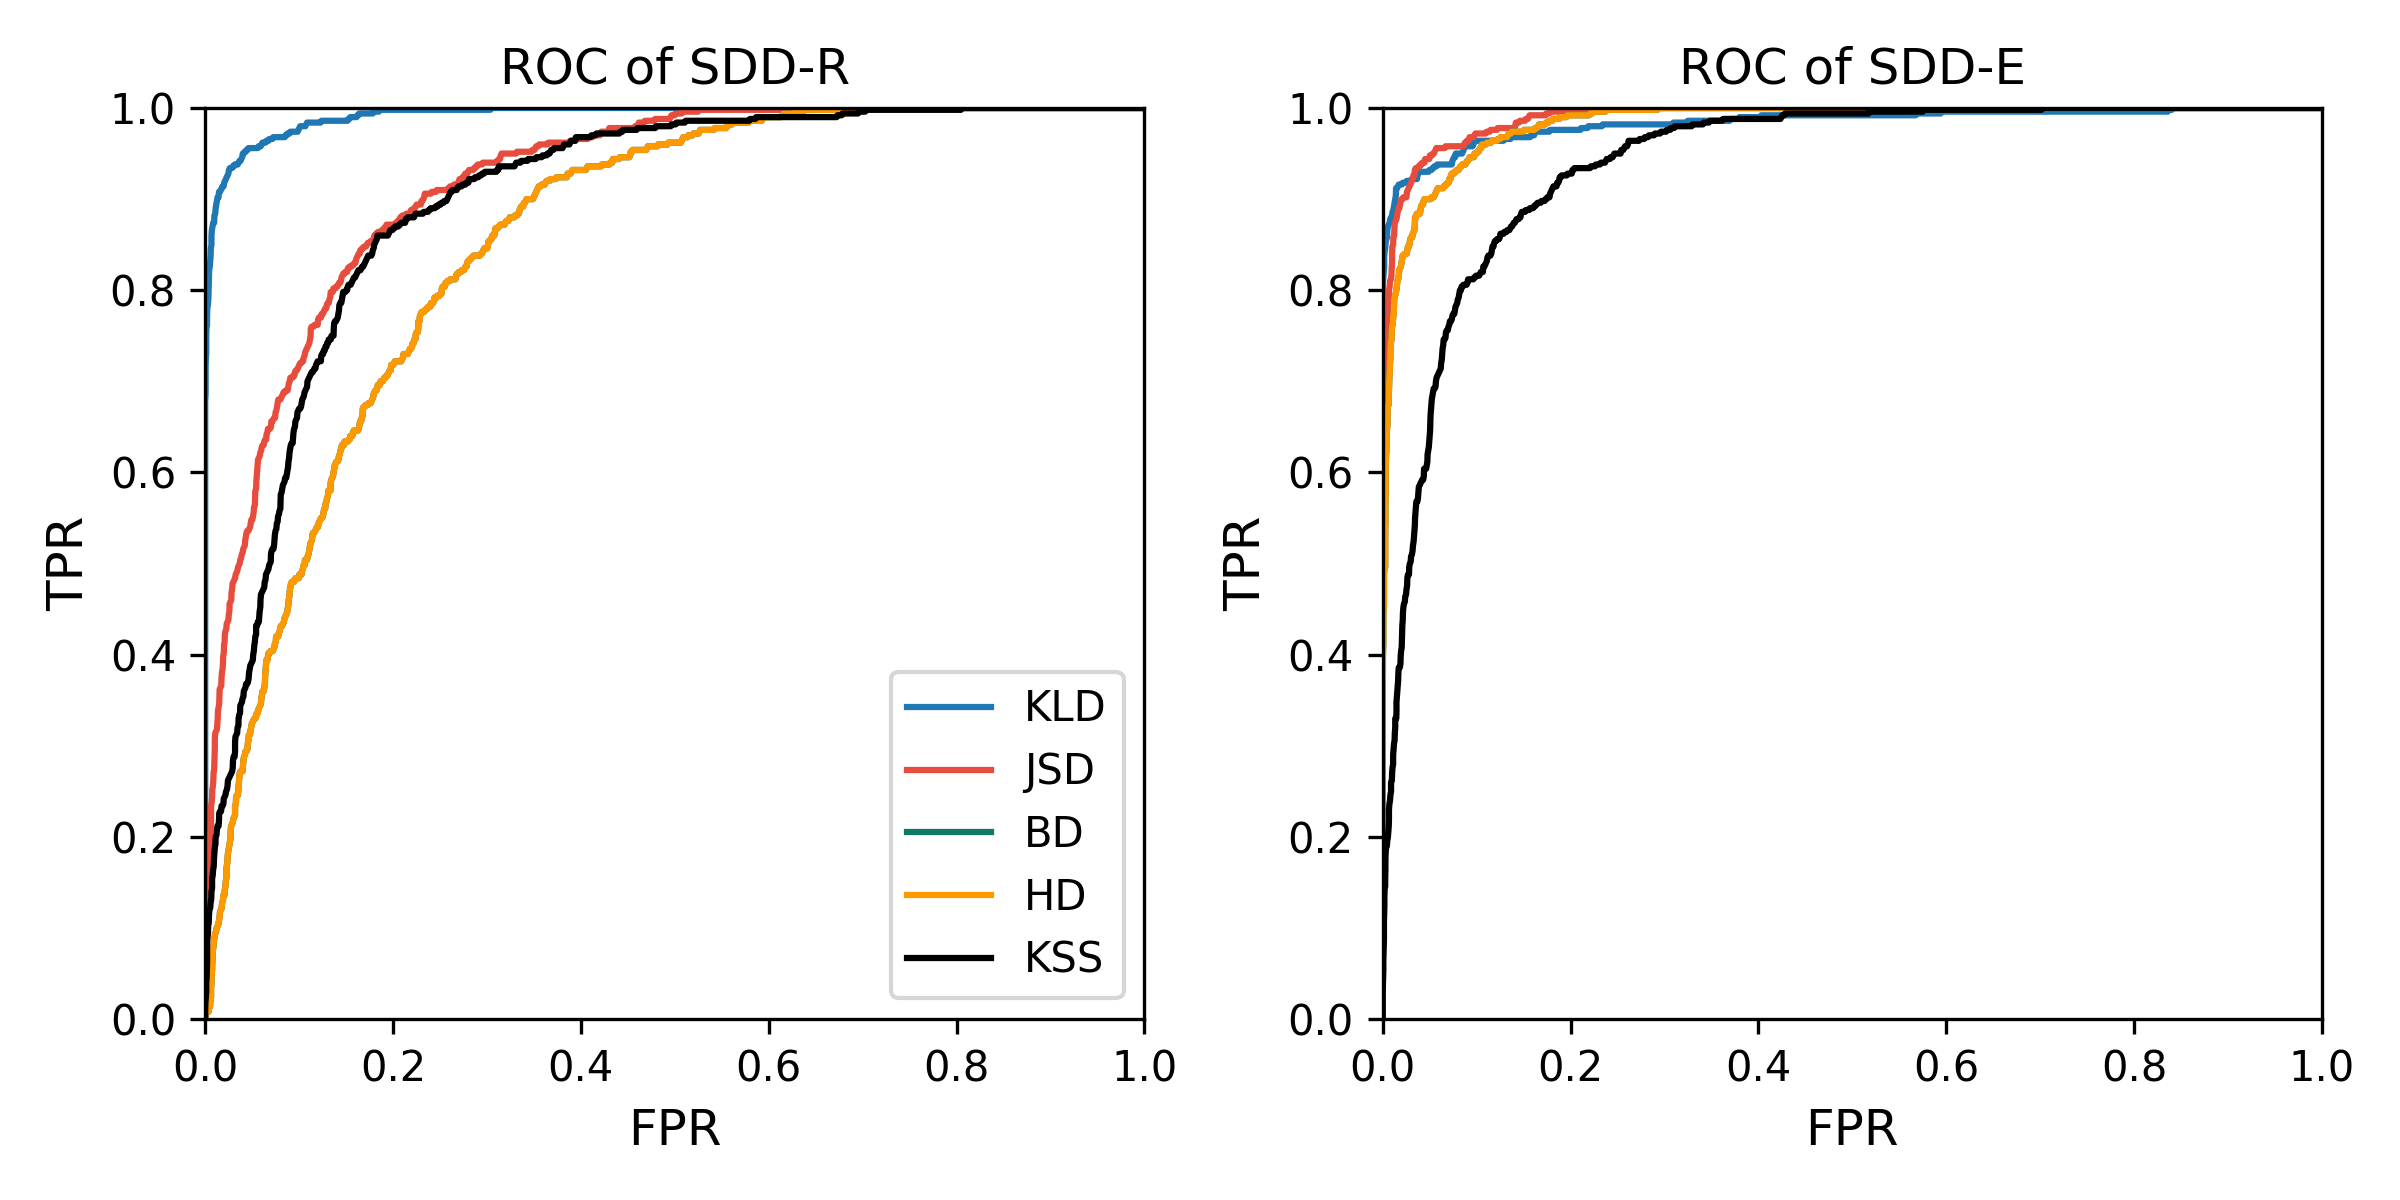
\includegraphics[width=.8\linewidth]{fig/ROCUnderDifferentMetrics.png}
				\captionof{figure}{ROC under Different Divergence Metric}
				\label{fig:divergence-metric-roc}
			\end{multicols}
		\end{sidewaystable}
		
		The last experiment was carried out on random-shaped distribution data set, with $alpha=0.1$ and rest parameters the same. Under different divergence metrics mentioned in section~\ref{sec:preliminaries}, F1 scores were calculated among all SDD algorithms and ROC curves were recorded on SDD-R and static SDD-E. Given that MGoF was defined specifically on Kullback-Leibler divergence, it cannot be tested in the same way. Results are shown in Fig.~\ref{fig:divergence-metric-f1} and Fig.~\ref{fig:divergence-metric-roc}.
		
		It is indicated that Jensen-Shannon divergence is suited to all techniques due to its symmetry. Kullback-Leibler divergence provides more evident differences when references were given. Bhattacharyya distance and Hellinger distance turned out almost as good as Jensen-Shannon divergence, but they consumed less time. Kolmogorov-Smirnov Statistic performed relatively poor since it considers only the largest gap between two distributions, which provides little information.
	
\end{document}